\documentclass[12pt]{article}
 
\usepackage[margin=1in]{geometry} 
\usepackage{amsmath,amsthm,amssymb}
\usepackage{graphicx}
\usepackage{epstopdf}
 
\newcommand{\N}{\mathbb{N}}
\newcommand{\Z}{\mathbb{Z}}
 
\newenvironment{exercise}[2][Exercise]{\begin{trivlist}
\item[\hskip \labelsep {\bfseries #1}\hskip \labelsep {\bfseries #2.}]}{\end{trivlist}}
\newenvironment{problem}[2][Problem]{\begin{trivlist}
\item[\hskip \labelsep {\bfseries #1}\hskip \labelsep {\bfseries #2.}]}{\end{trivlist}}
\usepackage{pdfpages}                    			    % Einbindung von PDF-Seiten
\usepackage{geometry}
\usepackage{courier}
\usepackage{color}
\usepackage{listings}
\definecolor{dkgreen}{rgb}{0,0.6,0}
\definecolor{gray}{rgb}{0.5,0.5,0.5}
\definecolor{ghostwhite}{rgb}{0.97, 0.97, 1.0}
\definecolor{vividviolet}{rgb}{0.62, 0.0, 1.0}

\lstset{language=Matlab,
   keywords={break,case,catch,continue,else,elseif,end,for,function,
      global,if,otherwise,persistent,return,switch,try,while},
   basicstyle=\ttfamily,
   keywordstyle=\color{blue},
   commentstyle=\color{dkgreen},
   stringstyle=\color{vividviolet},
   numbers=left,
   numberstyle=\tiny\color{gray},
   stepnumber=1,
   numbersep=10pt,
   backgroundcolor=\color{ghostwhite},
   tabsize=2,
   showspaces=false,
   showstringspaces=false}

\begin{document}
 
% --------------------------------------------------------------
%                         Start here
% --------------------------------------------------------------
 
\title{Weekly Homework 4}
\author{Benjamin Cramer, Julian G\"oltz\\
Brain Inspired Computing}
 
\maketitle
 
\begin{exercise}{4.1}
The high-conductance state in LIF neurons \\
\renewcommand{\labelenumi}{\alph{enumi})}
\begin{enumerate}
\item Let's introduce the total conductance which is given by:
  \begin{equation}
    g^{\text{tot}} = g_l + \sum_k g_k^{\text{syn}}
  \end{equation}
  Now consider using the expression for COBA synapses:
  \begin{equation}
    C_m \frac{du}{dt} = g_l (E_l - u) + I^{\text{ext}} + I^{\text{syn}} = g_l (E_l - u) + \sum_{\text{synapses }k}g_k^{\text{syn}}(E_k^{\text{rev}}-u) + I^{\text{syn}}
  \end{equation}
  We can now devide by $g^{\text{tot}}$ and obtain:
  \begin{align}
    \frac{C_m}{g^{\text{tot}}} \frac{du}{dt} &= \frac{g_lE_l + I^{\text{ext}} + \sum_{\text{synapses }k}g_k^{\text{syn}}E_k^{\text{rev}}}{g^{\text{tot}}} - \frac{g_lu + \sum_{\text{synapses }k}g_k^{\text{syn}}u}{g^{\text{tot}}} \\
                                             &= \frac{g_lE_l + I^{\text{ext}} + \sum_{\text{synapses }k}g_k^{\text{syn}}E_k^{\text{rev}}}{g^{\text{tot}}} - u
  \end{align}
  If we introduce:
  \begin{align}
    u_{\text{eff}} &= \frac{g_lE_l + I^{\text{ext}} + \sum_{\text{synapses }k}g_k^{\text{syn}}E_k^{\text{rev}}}{g^{\text{tot}}}\\
    \tau_{\text{eff}} &= \frac{C_m}{g^{\text{tot}}}
  \end{align}
  we are left with:
  \begin{equation}
    \tau_{\text{eff}} \frac{du}{dt} = u_{\text{eff}} - u
  \end{equation}
  \item The synaptic kernel $\epsilon(t)$ is given by:
  \begin{equation}
    \epsilon(t) = w\Theta(t)\exp{\left(-\frac{1}{\tau^{\text{syn}}}\right)}
  \end{equation}
  The solution of the integral is given by:
  \begin{equation}
    \int_0^\infty \epsilon(t)dt = \tau^{\text{syn}}w
  \end{equation}
  Since the the conductance-based model should reach the same membrane time constant as the current-based one we get:
  \begin{equation}
    \tau_m^{\text{curr}} = \frac{C_m}{\nu_{\text{HC}}\tau^{\text{syn}}w} \Leftrightarrow \nu_{\text{HC}} = \frac{C_m}{\tau_m^{\text{curr}}\tau^{\text{syn}}w} = 500000\text{\,Hz}
  \end{equation}
  Since the parameters for excitatory and inhibitory synapses are equal, we have to divide this solution by two since we are simulation the populations.
  \item A Gaussian fit is appropriate since in the high conductance state the input rate $\nu_{\text{HC}}$ has to be high. The central limit theorem guarantees that a sum of $n$ independent identically distributed random variables each with their moments $\mu$ and $\sigma$ converges almost surely to a Gaussian in the limit of large enough n ($n\rightarrow\infty$). For a high Poisson rate $\nu$ the number of events $n=\nu T$ can become arbitrarly large as well and therefore the central limit theorem applies. \\
  The value of $\langle u \rangle$ is equal to the leak potential since excitatory and inhibitory inputs are balanced and the distance towards the reversal potentials $E_{\text{rev}}^{\text{exc}}$ and $E_{\text{rev}}^{\text{inh}}$ are equal.
  The Gaussian fit for the distribution of conductances leads to a mean of $\langle g^{\text{tot}} \rangle = 253$\,nS. The theoretical predictions leads to $\langle g^{\text{tot}} \rangle = 250$\,nS, so the theoretical prediction and the simulated data agree quite well.

  \center{
  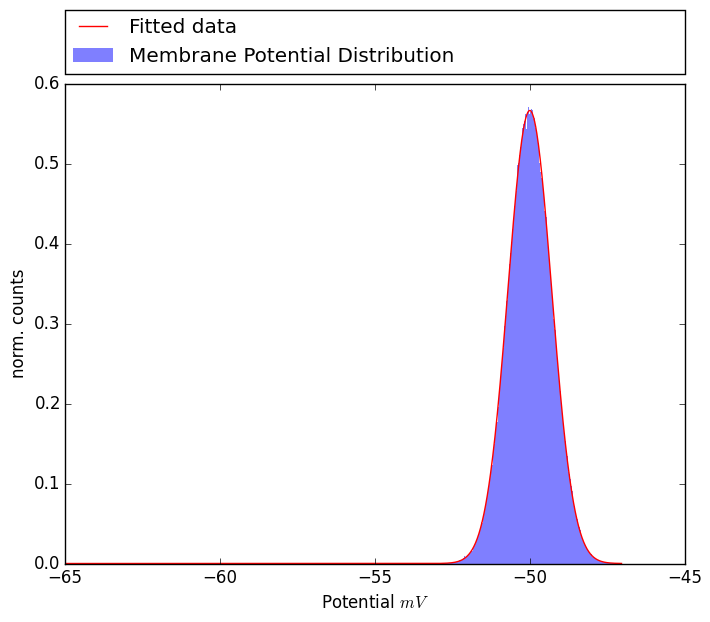
\includegraphics[width=4.4in]{codes/excercise1_pot}

  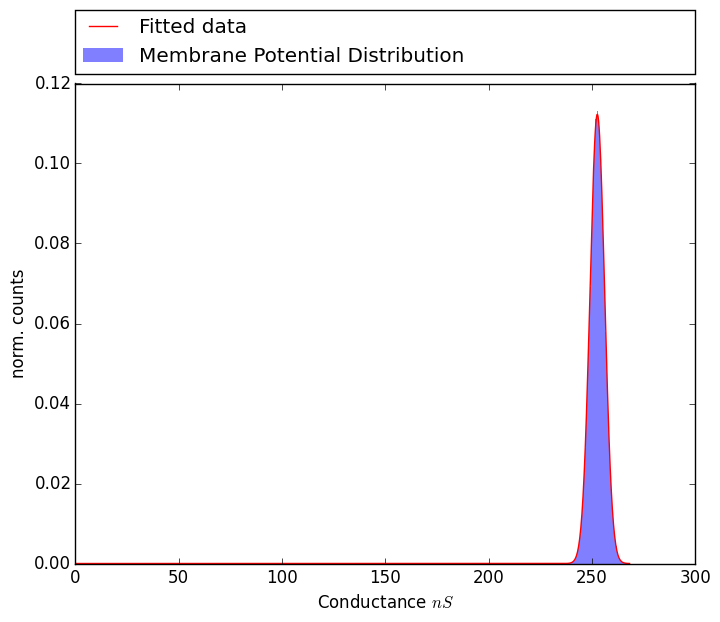
\includegraphics[width=4.4in]{codes/excercise1_cond}}

\end{enumerate}

\end{exercise}

\begin{exercise}{4.2}
$f-I$ curves \\
\renewcommand{\labelenumi}{\alph{enumi})}
\begin{enumerate}
\item From the lecture we know:
  \begin{equation}
    \nu(I^{\text{ext}}) = \left(\tau_{\text{ref}} + \tau_m \log{\frac{\rho - E_l - \frac{I^{\text{ext}}}{g_l}}{\theta - E_l - \frac{I^{\text{ext}}}{g_l}}}\right)^{-1}
  \end{equation}
  The asymptotic behavior of $\nu(I^{\text{ext}})$ for $I^{\text{ext}}\rightarrow \infty$ in the limit of $\tau_{\text{ref}}\rightarrow 0$ is given by:
  \begin{align}
    \lim_{I^{\text{ext}}\rightarrow \infty} \lim_{\tau_{\text{ref}}\rightarrow 0} &\left(\tau_{\text{ref}} + \tau_m \log{\frac{\rho - E_l - \frac{I^{\text{ext}}}{g_l}}{\theta - E_l - \frac{I^{\text{ext}}}{g_l}}}\right)^{-1} \\
                                                                                  &=\lim_{I^{\text{ext}}\rightarrow \infty}\left(\tau_m \log{\frac{\rho - E_l - \frac{I^{\text{ext}}}{g_l}}{\theta - E_l - \frac{I^{\text{ext}}}{g_l}}}\right)^{-1} \\
                                                                                  &\rightarrow \infty
  \end{align}
\item Since it is not possible to choose an arbitrary small refractory time (time step), we choose several small numbers which confirms the divergence of result of exercise a). As an example the next plot shows a simulation with an value of $\tau_{\text{ref}}=0.1$.

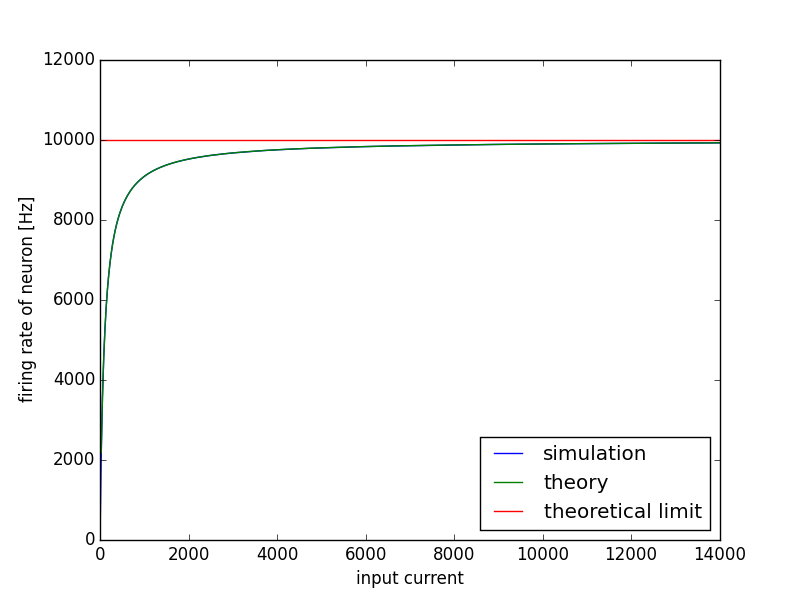
\includegraphics[width=5.2in]{codes/excercise2_01}

The next plot shows the results of a setup with $\tau_{\text{syn}} = 5.0$\,ms

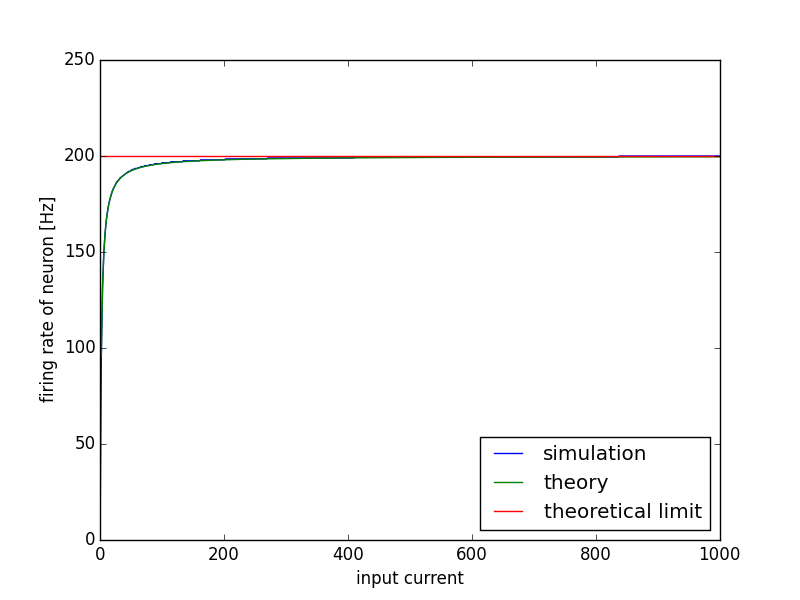
\includegraphics[width=5.2in]{codes/excercise2_5}

\end{enumerate}

\end{exercise}

\end{document}